\section{Music source separation}
\label{sec:background}

\begin{figure}
  \centering
  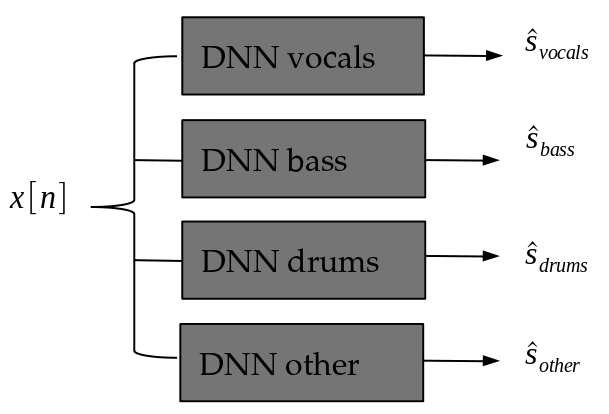
\includegraphics[width=0.5\columnwidth]{mss-basic.png}
  \label{fig:mss-basic}
  \caption{DNN could predict music sources sample per sample}
\end{figure}

In this Section, we present the general methods for separating musical
sources using neural networks.
As illustrated in the Figure~\ref{fig:mss-basic}, one tentative consists
in predicting a source $\hat{s}$ given a sample of the mixture signal $x[n]$.
Unfortunately, this task is impossible to achieve:
given only one sample and no context, no pattern can be learned.

Bringing more context means that the neural network is fed
 with a sequence of samples $(x[n+i])_{i\in [-N, N]}$.
Music patterns, such as fading, last roughly 5 seconds.
 With a sample rate of 44.1 kHz, the input sequence would have a length of $441k$ samples.
At that size, the curse of dimensionalityi~\cite{mallat} makes it difficult to learn patterns.



\subsection{Short-term Fourier transform}

Instead, it seems preferable to help the neural network to
figure out some invariances using pre-processing steps.
A widely employed in audio consists in transforming an audio signal
into the short-term Fourier transform (STFT).
The STFT is particularly employed in audio processing, as the signal decomposition is varying around the time axis.
It is directly derived from the Fourier transform by employing a window function of a short window (typically 20 ms)
and a delay function:


$$\mathbf{STFT}\{x(t)\}(\tau,\omega) = X(\tau,\omega) = e^{j\omega t/2}\int_{-\infty}^\infty {x(t)w(t-\tau)e^{-jwt}dt}.$$

A possible window, that we will use thereafter, is the Gaussian function, parametrized by $\lambda$:
$$h(t) = \lambda^{-1/2}\pi^{-1/4}e^{-t^2/(2\lambda^2)}.$$

The STFT of a signal is then a two dimensional and complex signal:
$$X(\omega, \tau) = |X|(\omega, \tau) e^{j\phi(\omega, \tau)},$$
with $\phi$ and $|X|$ the phase and the amplitude.
Numerical audio signals are sampled for discrete time steps $n$, and in this case:
$$\mathbf {STFT} \{x[n]\}(m,\omega ) = X(m,\omega )=e^{j\omega t/2}\sum _{n=-\infty }^{\infty }x[n]w[n-m]e^{-j\omega n}.$$


\begin{figure}
  \centering
  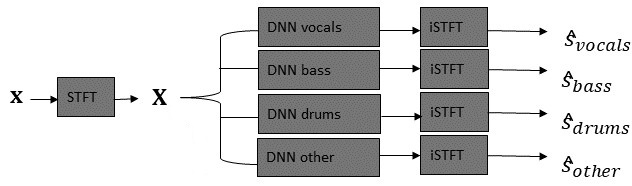
\includegraphics[width=0.9\columnwidth]{mss-stft-2}
  \label{fig:mss-stft}
  \caption{Models are more easily trained when inputs are transformed with an STFT.}
\end{figure}

Using an STFT, one solution to the music separation problem is to fed the
DNN with the amplitude and the phase of the mixture signal,
as illustrated in Figure~\ref{fig:mss-stft}.
In this case, the DNN predict the amplitude and the phase of each source.
Then the inverse STFT (iSTFT) is applied on the predicted amplitude and phase to reconstruct the source.
The use of STFT is motivated by two reasons.

\begin{itemize}
  \item Patterns are more easily identifiable in the spectrograms, for which trained experts are able to recognize speechs;
  \item Getting around the curse of dimensionality requires to reduce the input's size. Using the STFT, the time context can be strongly reduced going from a window of 10s to a fraction of seconds. Thereafter, the setup uses a time context of 11 and 2049 frequency bins, such that the input's size becomes around 45 k.
\end{itemize}


\subsection{Sharing the phase of the mixture signal}

As observed by~\cite{chandna2017monoaural}, \cite{jansson2017singing},
a neural network in the format of the Figure~\ref{fig:mss-stft} can hardly
predict the phase, because of its intrinsic discontinuous shape.

\begin{figure}
  \centering
  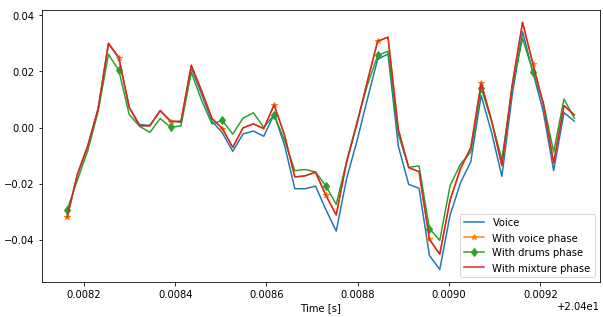
\includegraphics[width=0.9\columnwidth]{approx-phase}
  \label{fig:approx-phase}
  \caption{Comparison between the voice source, the signal reconstructed after an STFT transformation, the signal reconstructed with the phase of the mixture, and with the phase of the drums source}
\end{figure}

In the context of music source separation, it is generally assumed
that the phase of the mixture signal is the same than each source's phase.
This approximated is illustrated in Figure~\ref{fig:approx-phase}. An excerpt of the voice source is compared with other signals: the same signal once the STFT and its inverse iSTFT were applied, the voice signal reconstituted with the mixture phase and the with drums source. It appears that the signal is slightly modified by the STFT operation, but it is invariant to the mixture's phase. If the mixture's phase seems to include other phase, the approximation is more visible when reconstructing the signal using the drums' phase.
One explanation is that instruments are playing in rhythm.
Some authors~\cite{mowlaee2015harmonic},~\cite{gerkmann2015phase} argue against this approximation, particularly in the context of speech enhancement.

Subsequently, the problem of estimating sources is simplified by the estimating the magnitude of the STFT of each source, as illustrated in the Figure~\ref{fig:mss-amp}.


\begin{figure}
  \centering
  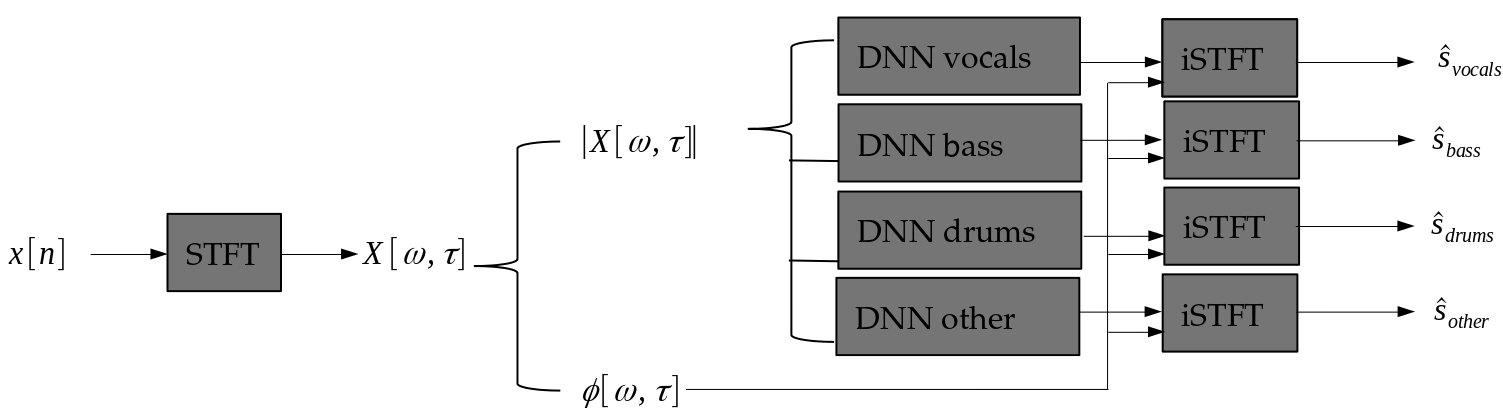
\includegraphics[width=0.9\columnwidth]{mss-amp}
  \label{fig:mss-amp}
  \caption{The DNN is trained to predict only the amplitude of a source signal audio.}
\end{figure}




\section{Using the phase to predict the magnitude}

The neural network presented in the Figure~\ref{fig:mss-amp} illustrates the
structure of state-of-the-art architectures~\cite{chandna2017monoaural}.
The goal of Muth et al. research consists in using the phase to improve the prediction
of the magnitude.
Unfortunately, it seems unfeasible to use directly the phase when predicting
the magnitude of each source. The authors tried to fed a network composed of
a few fully connected layers with the magnitude and the phase of the mixture
signal to order to predict the magnitude of one source. They observe that
their optimizer algorithm tends to lower to zero the weights connecting
the phase features to the rest of the network.

Instead of using the phase as an input to the neural network, one could use
the derivatives of the phase as shown in the Figure~\ref{fig:nn}
Following the work of \cite{auger2012phase}, it exists a relation
between the amplitude and the phase of the STFT of a signal.
The analytical expression is simplified for the case of a Gaussian window with a given-width $\lambda$:

\begin{equation}
    \left\{
        \begin{array}{ll}
            \frac{\partial }{\partial t}\phi(\omega, \tau) &= \lambda^{-2}   \frac{\partial}{\partial \omega} \log(A(\omega, \tau)) + \frac{\omega}{2} \\
            \frac{\partial d}{\partial \omega}\phi(\omega, \tau) &= -\lambda^{-2}   \frac{\partial}{\partial t} \log(A(\omega, \tau)) - \frac{t}{2}
        \end{array}
    \right.
\end{equation}

\begin{figure}
  \centering
  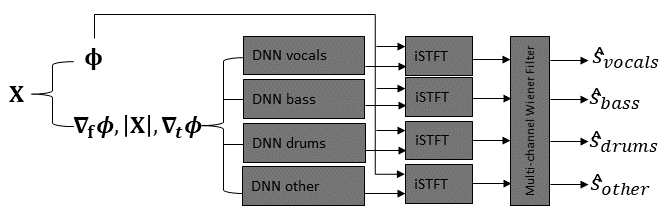
\includegraphics[width=0.8\columnwidth]{nn.png}
  \label{fig:nn}
  \caption{Architecture of the neural network}
\end{figure}


While using $\nabla_f \phi$ and
$\nabla_t \phi$ instead of $\phi$ seems reasonable,
it is worth to note that neural networks tend to over-fit on the training set
when given correlated inputs.
The derivatives are numerically obtained from first-order approximations:
$$\nabla_\tau \phi(k, m) = \phi(k, m) - \phi(k,m-1)$$
$$\nabla_\omega \phi(k, m) = \phi(k, m) - \phi(k-1,m)$$

The amplitudes of the neural networks are predicted up to a scale, such that the authors used a multi-channel Wiener filter at the output.
All in all, the neural network's architecture proposed by the author is
illustrated in the Figure~\ref{fig:orig-nn}. Considering a sample $x[n]$ of the
mixture signal, we fed the neural network with the magnitude, and the derivatives
 of the phase for all frequency bins and for a time context of 11 other samples.
 The presented Figure is extracted from the original article.
 It seems a concatenation layer is missing.
Although the network is not very deep, it is particularly wide,
since the model achieves more than 70 millions of parameters.

\begin{figure}
  \centering
  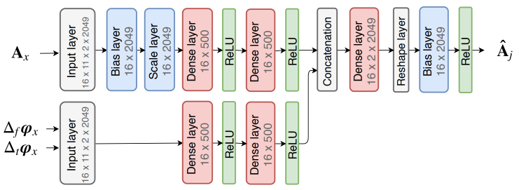
\includegraphics[width=0.8\columnwidth]{orig-nn.png}
  \label{fig:orig-nn}
  \caption{Solution of Muth et al. to separate musical sources.}
\end{figure}


\subsection{Correction in the distribution of the phase features.}

\begin{figure}
	  \centering
	    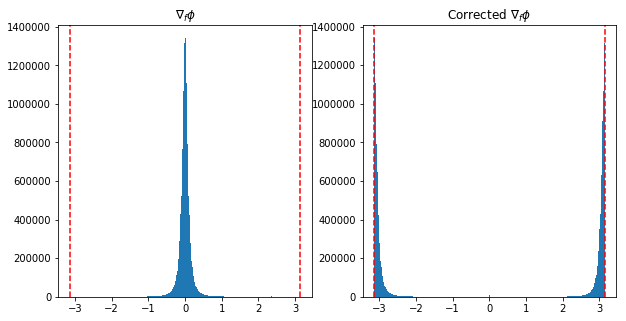
\includegraphics[width=0.9\columnwidth]{dist-df.png}
	      \label{fig:dist-df}
	        \caption{Distribution of $\nabla_f\phi$ and its correction.}
	\end{figure}


\begin{figure}
	  \centering
	    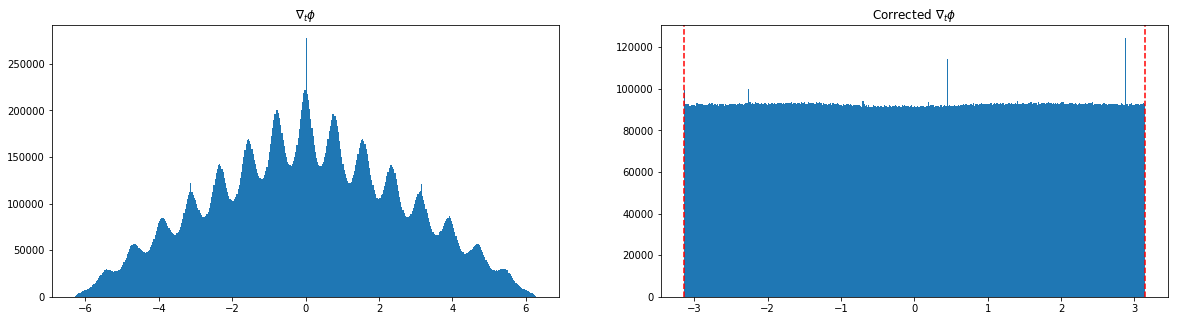
\includegraphics[width=1.0\columnwidth]{dist-dt.png}
	      \label{fig:dist-dt}
	        \caption{Distribution of $\nabla_f\phi$ and its correction.}
	\end{figure}

Additional pre-processing steps are suggested by the authors.
Pre-processing is used in neural networks to help an optimization algorithm
to find symmetries in the training set. Pre-processing is all the more important when the dataset is small.
As seen in the Figures~\ref{fig:dist-df} and \ref{fig:dist-dt},
the distributions of $\nabla_f \phi$ and $\nabla_t \phi$ are biased.
We observe that $\nabla_f \phi$ has a systematic shift of $\pi$,
whereas $\nabla_\tau \phi$ has a shift of $2\pi k\frac{n_0}{N}$,
where $n_0$ is the hop size, namely the number of taps between two samples $k$ and $k+1$.

The shift of $\nabla_t \phi$ is explained by the shift theorem
of the discrete Fourier transform \cite{smith2007mathematics}:
$$x(n-n_0) \xrightarrow{\text{DFT}}
e^{j\frac{2\pi}{N}kn_0}X(k).$$
